\documentclass[a4paper, 12pt]{article}
\usepackage[utf8]{inputenc}
\usepackage{graphicx}
\usepackage{amsmath}

\title{COMP6212 Lab 1}
\author{James Robinson}

\begin{document}

	\maketitle

	\section{Efficient Mean-Variance frontier}

	\subsection{Randomly-selected portfolio analysis}

	100 portfolios were randomly selected and analysed using the following procedure for each portfolio:

	\begin{itemize}
		\item Construct a vector of length 3, where each element is a random number between 0 and 1,
		\item Divide the vector by its $L^1$-norm to produce a portfolio $X$ with $\sum_{i=1}^3{X_i} = 1$,
		\item Calculate the expected return $E = \sum_{i=1}^3 X_i \mu_i$,
		\item Calculate the expected variance $V = \sum_{i=1}^3 \sum_{j=1}^3 X_i X_j \sigma_{ij}$.
	\end{itemize}

	The efficient frontier for this 3 asset model was plotted using the MATLAB \texttt{frontcon} function, and an E-V plot of the 100 randomly selected portfolios was plotted on the same axes (see figure~\ref{fig:p1a}). N.B. the orientation of the axes and that the X axis shows standard deviation instead of variance.

	\begin{figure}
		\begin{center}
			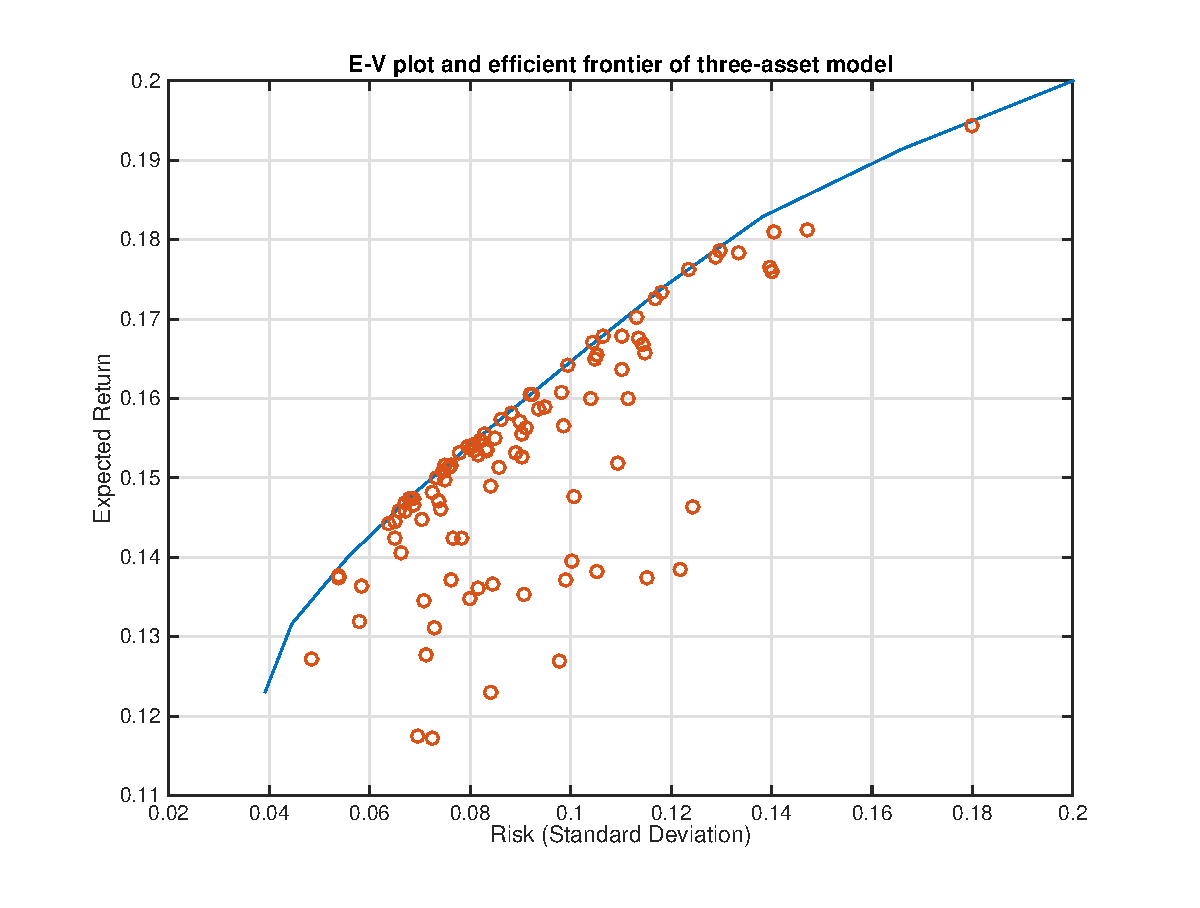
\includegraphics[width=0.75\linewidth]{figures/p1a.eps}
		\end{center}
		\caption{E-V plot of 100 randomly selected portfolios against efficient frontier for three-asset model}
		\label{fig:p1a}
	\end{figure}

	Three two-asset markets were constructed from this 3 asset model by removing the corresponding values from the mean vector and the covariance matrix, and the same procedure detailed above was followed to produce E-V plots and efficient frontiers for each model (see figure~\ref{fig:p1b}). Of note is the fact that under the two-asset model, all of the randomly selected portfolios fall exactly on the edge of the attainable region. In addition, in two-asset models 1 and 3 the covariance matrix contains negative values, meaning that some portfolio combinations fall below the efficient frontier. In two-asset model 2 every element of the covariance matrix is positive, and so every portfolio falls exactly upon the efficient frontier.

	\begin{figure}
		\begin{center}
			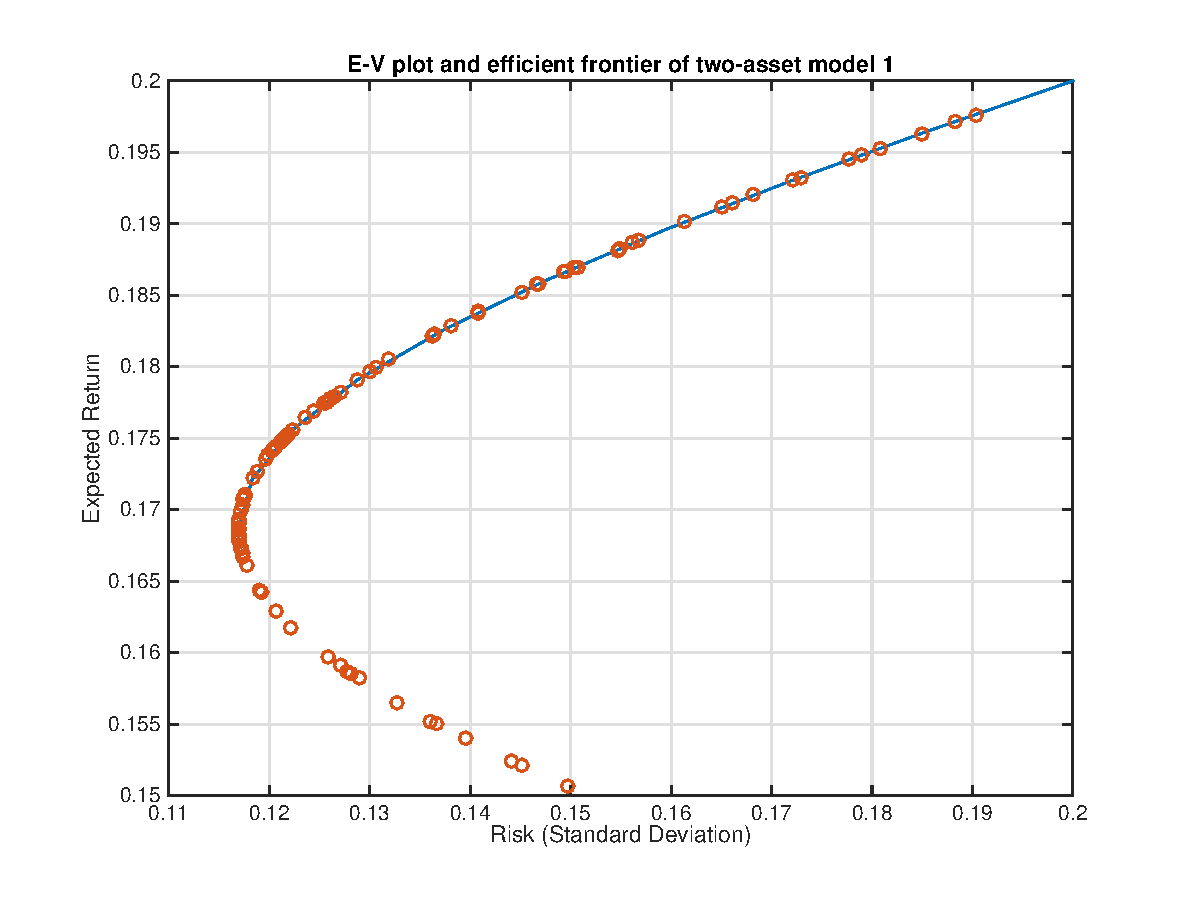
\includegraphics[width=0.3\linewidth]{figures/p1b_1.eps}
			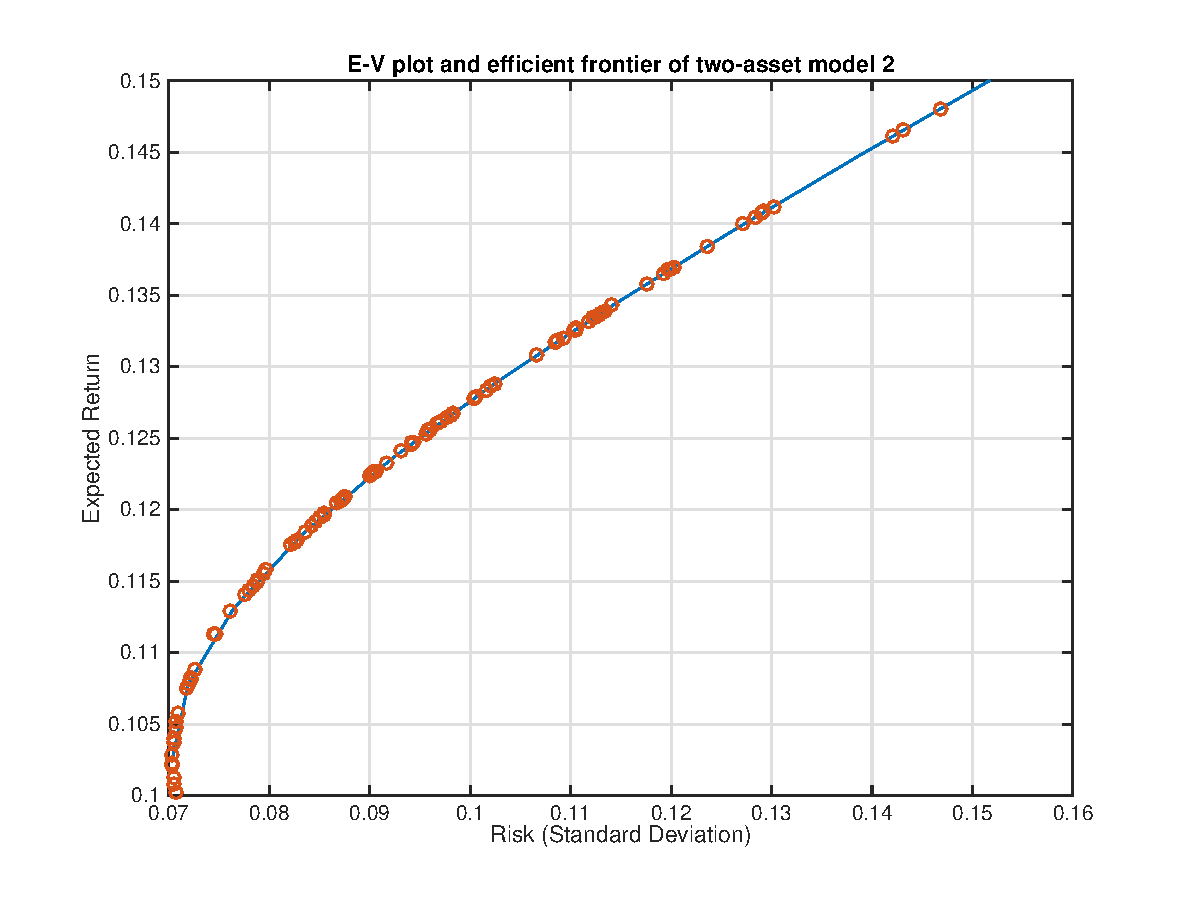
\includegraphics[width=0.3\linewidth]{figures/p1b_2.eps}
			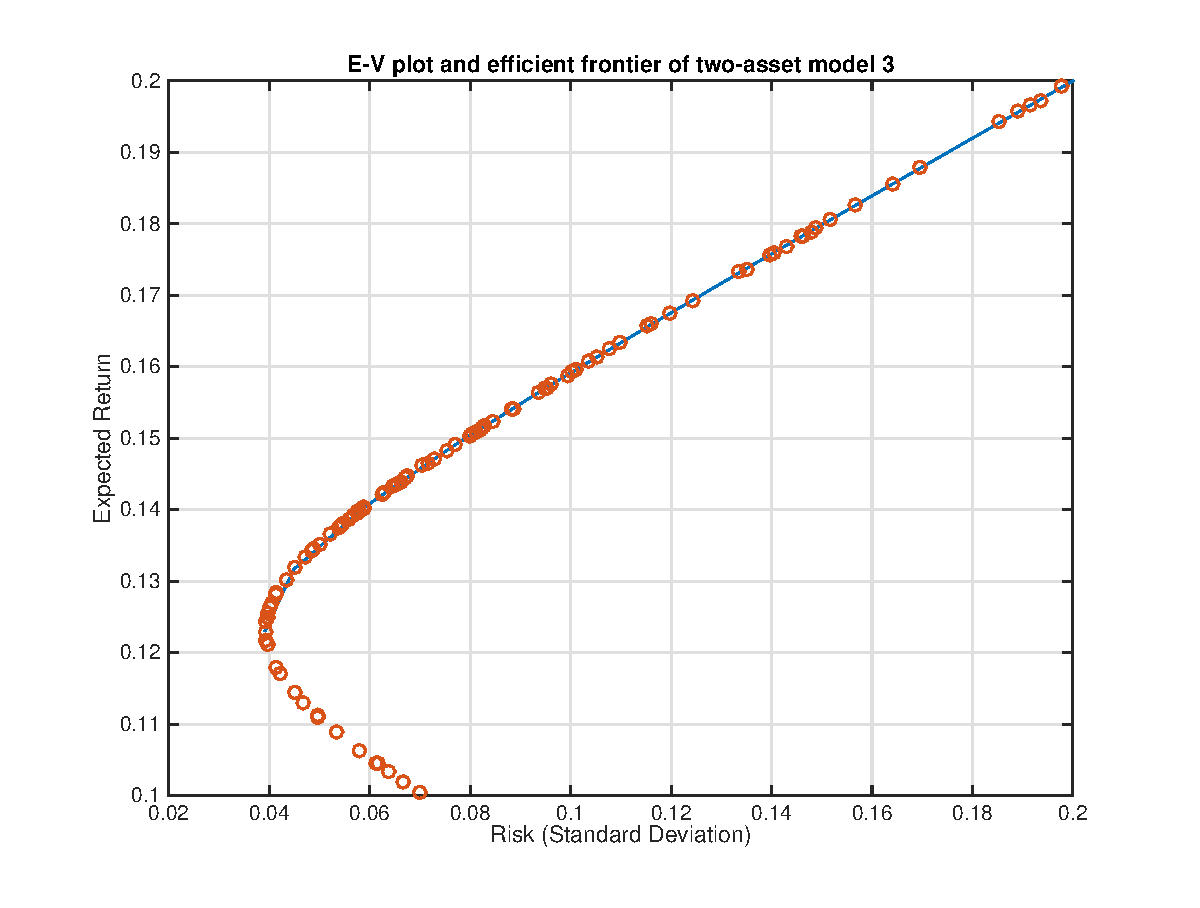
\includegraphics[width=0.3\linewidth]{figures/p1b_3.eps}
		\end{center}
		\caption{E-V plots of 100 randomly selected portfolios against efficient frontier for three two-asset models, taken pairwise from three-asset model}
		\label{fig:p1b}
	\end{figure}

	\subsection{Efficient frontier plotting}

	The NativeMV function works by first finding both the maximum achievable return and the return associated with the minimum possible variance. Given a vector of mean returns $\bar{\mathbf{r}}$, the portfolio $\mathbf{w}$ that achieves the maximum possible return can be found by solving the following objective function:

	\[\text{max } \mathbf{w}^T \bar{\mathbf{r}} \text{ subject to } \sum_{i=1}^N w_i = 1, w_i \geq 0\]

	This is a trivial linear programming problem whose solution is the portfolio solely consisting of the single asset with the highest expected return. However, the \texttt{NativeMV} function uses the \texttt{linprog} function so that additional constraints may be placed upon the problem, thus making it non-trivial to solve.

	\subsection{Modification of NativeMV}

	The \texttt{linprog} function call used by \texttt{NativeMV} to find the maximum achievable return was replaced with CVX, using the objective function detailed in the previous section. The return associated with the minimum possible variance was determined by solving this objective function:

	\[\text{min } \mathbf{w}^T \mathbf{\Sigma w} \text{ subject to } \sum_{i=1}^N w_i = 1, w_i \geq 0\]

	Finally, the set of efficient portfolios was traced by replacing the final call to \texttt{quadprog} with the following objective function:

	\[\text{min } \mathbf{w}^T \mathbf{\Sigma w} \text{ subject to } \mathbf{w}^T \bar{\mathbf{r}} = \bar{r}_T, \sum_{i=1}^n w_i = 1, w_i \geq 0\]

	Efficient frontiers for some sample data traced by \texttt{NativeMV} and a modified version of the same function using CVX instead of \texttt{linprog} and \texttt{quadprog} are shown on the same axes in figure~\ref{fig:p1d}. Note that the frontiers produced by the two different implementations are completely identical. The implementation using CVX took an order of magnitude longer to compute the efficient frontier, however.

	\begin{figure}
		\begin{center}
			\includegraphics[width=0.75\linewidth]{figures/p1d.eps}
		\end{center}
		\caption{Efficient frontier produced by NativeMV}
		\label{fig:p1d}
	\end{figure}

	\section{Evaluation of performance}

	Three years of historical data for 3 of the FTSE 100 constituent stocks were obtained from Yahoo Finance. Missing days in the historical data were filled in by carrying over the adjusted closing price from the previous day, producing datasets of equal length. The MATLAB \texttt{tick2ret} function was used to transform this price data into returns time series', producing a $T$x$N$ matrix of returns $R$.

	The historical data was used with $T = 500$ to estimate the means and covariance matrix for the first half of the dataset in the following way:

	\[
		\hat{\mu} = \frac{1}{T} \sum_{t=1}^T \mathbf{r}(t) = \begin{pmatrix}
			-0.0011 & 0.0010 & 0.0007
		\end{pmatrix}
	\]

	\[
		\hat{\Sigma} = \frac{1}{T} \sum_{t=1}^T (\mathbf{r}(t) - \hat{\mu})^T (\mathbf{r}(t) - \hat{\mu}) = 1 \times 10^{-3} \begin{pmatrix}
			0.3113 & 0.0404 & 0.0820 \\
			0.0404 & 0.0987 & 0.0374 \\
			0.0820 & 0.0374 & 0.1804
		\end{pmatrix}
	\]

	The CVX toolkit was then used to find the portfolio with the highest possible return given a maximum standard deviation of 0.0088 by solving the following objective function:

	\[
		\max_{\pi} \pi^T \mu \text{ subject to } \pi^T \Sigma \pi \leq 0.0088^2
	\]

	\[
		\pi^T = \begin{pmatrix}
			0.0776 & 0.660 & 0.262
		\end{pmatrix}
	\]

	In addition, a naïve 1/N portfolio was selected to compare this efficient portfolio against:

	\[
		\pi^T = \begin{pmatrix}
			\frac{1}{3} & \frac{1}{3} & \frac{1}{3}
		\end{pmatrix}
	\]

	A return time series $R\pi$ was calculated over the second half of the dataset ($t = 501$ to $1000$) for each portfolio, and MATLAB's \texttt{cumsum} function was used to produce cumulative sums for each, shown over time in figure~\ref{fig:p2_cumulative_return}. The Sharpe ratios for each portfolio were also calculated using MATLAB's \texttt{sharpe} function \emph{assuming no risk-free asset}: the efficient portfolio had a ratio of 0.767, and the 1/N portfolio had a ratio of 0.0504. Note that because no risk-free asset was chosen in this example the Sharpe ratios may not be directly compared against real-world examples (although they can still be used to compare the relative efficiency of the portfolios in this hypothetical scenario).

	In this particular scenario, the efficient portfolio performed slightly better than the 1/N one, producing a higher return at a higher Sharpe ratio.

	\begin{figure}[b!]
		\begin{center}
			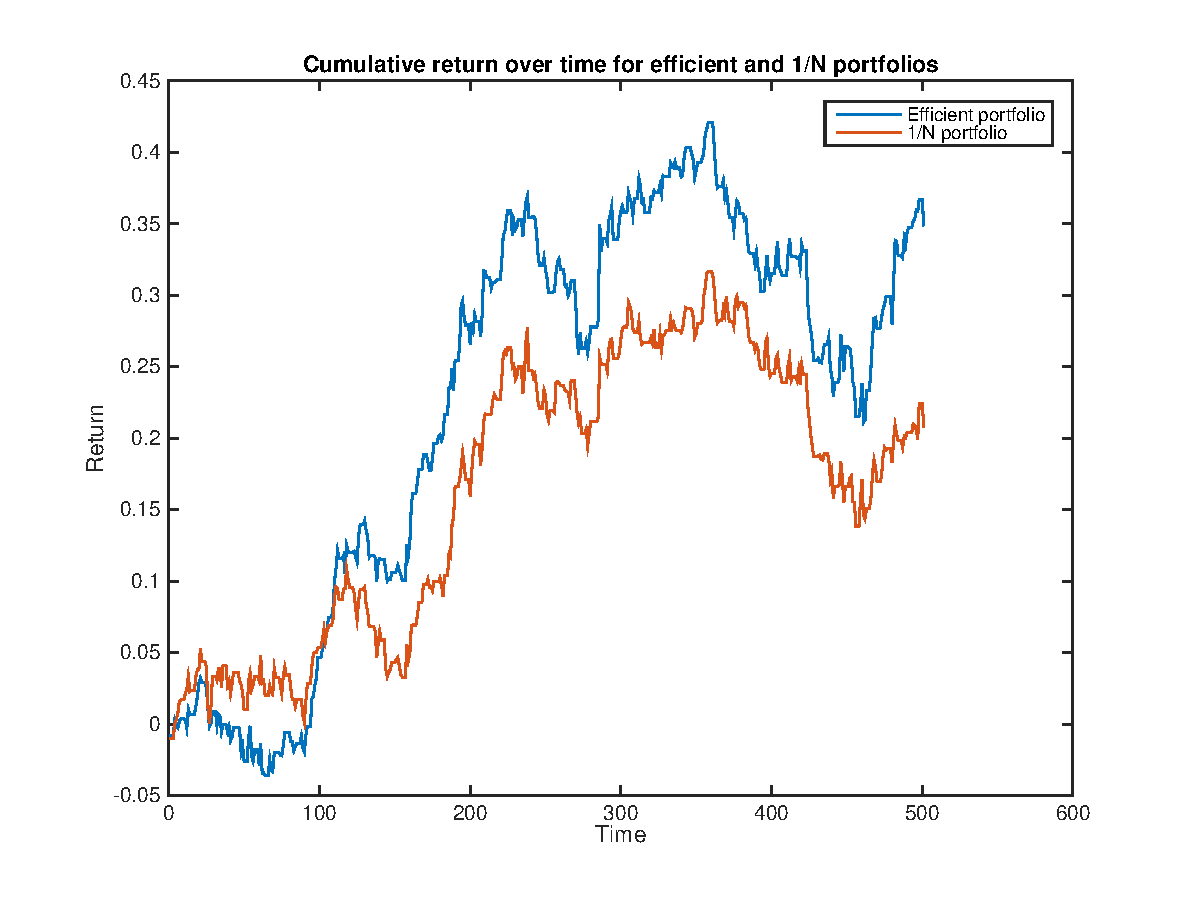
\includegraphics[width=0.75\linewidth]{figures/p2_cumulative_return.eps}
		\end{center}
		\caption{Cumulative returns of efficient and 1/N portfolios over time}
		\label{fig:p2_cumulative_return}
	\end{figure}

	\section{Greedy and sparse index tracking}

	Three years of historical data for the FTSE 100 index and 30 of its constituent stocks were obtained and processed in the same manner as in the previous section. The MATLAB \texttt{tick2ret} function was used to transform this price data into returns time series', producing a $T$x$1$ vector $\mathbf{y}$ of returns for the FTSE 100 index, and a $T$x$N$ matrix $\mathbf{R}$ of returns for constituent stocks.

	A greedy search algorithm for index tracking was then implemented, beginning with an empty portfolio and at each step adding to the portfolio the asset that produces the lowest value $\|\mathbf{y} - \mathbf{Rw}\|_2^2$ for the portfolio. This process was repeated 6 times to produce a 6 asset portfolio, shown in figure~\ref{fig:p3a}.

	\begin{figure}[b!]
		\begin{center}
			\includegraphics[width=0.45\linewidth]{figures/p3a_portfolio.eps}
			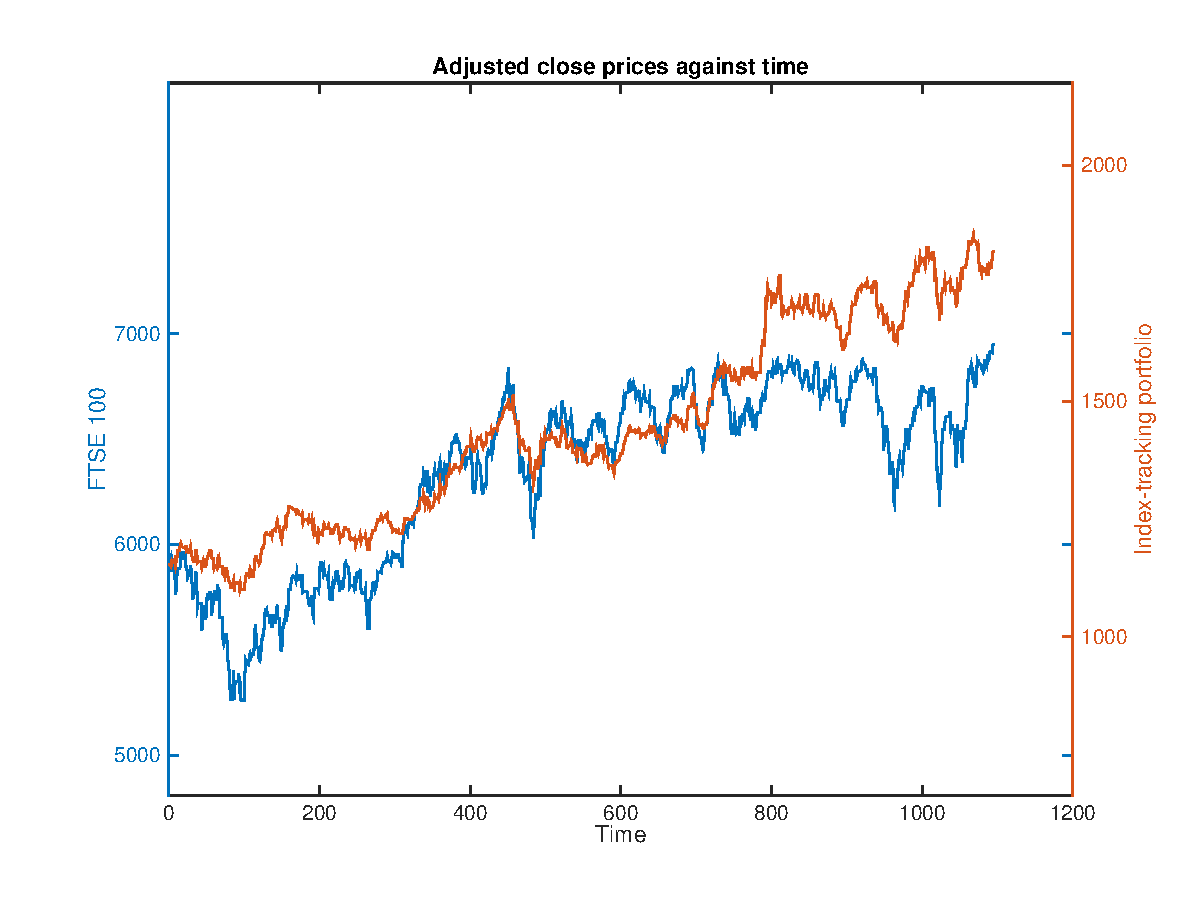
\includegraphics[width=0.45\linewidth]{figures/p3a_ticker.eps}
		\end{center}
		\caption{Index tracking portfolio selected via greedy search}
		\label{fig:p3a}
	\end{figure}

	A second portfolio was constructed using the technique of $L^1$-regularization. The CVX toolkit was used to solve the objective function:

	\[\mathbf{\hat{w}} = \min_{w} [\|\mathbf{y} - \mathbf{Rw}\|_2^2 + \tau \| \mathbf{w} \|_1]\]

	A value of $\tau = 0.09$ was selected to produce a 6 asset portfolio, shown in figure~\ref{fig:p3b}.

	\begin{figure}
		\begin{center}
			\includegraphics[width=0.45\linewidth]{figures/p3b_portfolio.eps}
			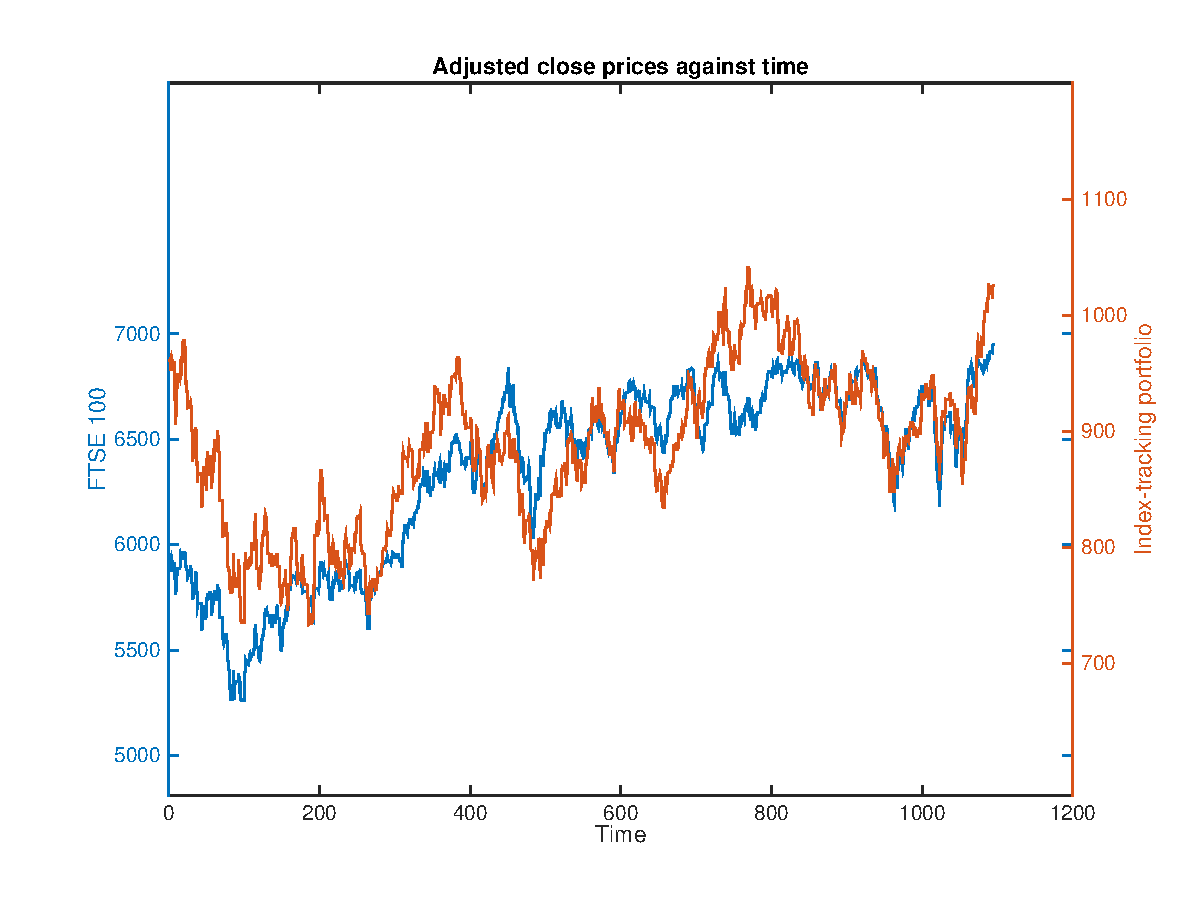
\includegraphics[width=0.45\linewidth]{figures/p3b_ticker.eps}
		\end{center}
		\caption{Index tracking portfolio selected via $L^1$-regularization}
		\label{fig:p3b}
	\end{figure}

	Both methods performed significantly worse than a dense portfolio, producing $\|\mathbf{y} - \mathbf{Rw}\|_2^2$ values of 0.0115 and 0.0668 respectively (compared to a value of 0.0026 when constructing a dense portfolio via $L^1$-normalization with $\tau = 0$). However, this performance penalty comes with the benefit of reducing the number of held assets required to track the index by a significant margin, which can help to minimize transaction costs. Particularly surprising was the discovery that the portfolio produced by $L^1$-normalization tracked the index less precisely than the greedy algorithm.

	\section{Discussion of Lobo et al.}

	Lobo et al. describe a method of incorporating transaction costs into the optimisation of portfolio adjustment. They propose an objective function that maximizes expected return while taking transaction costs into account. The function is detailed on page 11 of the paper, and the constraints are as follows:

	\begin{enumerate}
		\item The sum of the transaction costs must not exceed the value gained from the transactions
		\item Transaction costs must be positive
		\item Short-selling constraint: the amount owed must not exceed a certain threshold
		\item Ensures that total wealth will never fall below $W^{low}$ with a given confidence
	\end{enumerate}

\end{document}
